\begin{enumerate}[label=\thesubsection.\arabic*,ref=\thesubsection.\theenumi]
\item The two opposite vertices of a square are $\vec{A}(–1, 2)$  and $ \vec{C}(3, 2)$. Find the coordinates of the other two vertices.
\\
\solution
	\begin{align}
\vec{C} - \vec{A} = \myvec{
4\\
0
} \equiv 
\myvec{
1\\
0
},\,
\implies \phi= 0\degree
\end{align}
		where
$\phi$ is the angle made by $AC$ with the x-axis.
Also, the diagonal
\begin{align}
	d = \norm{\vec{C}-\vec{A}} = 4
\end{align}
\begin{enumerate}
	\item We start with  the square in \figref{fig:7/4/4/4Fig3},
 with vertices as columns of the matrix
\begin{align}
	\vec{y} = \frac{d}{\sqrt 2}\myvec{0 & 1 & 1 & 0 \\ 0 & 0 & 1 & 1}
\end{align}
	in \eqref{eq:conic_affine}.
\item The next square, obtained as 
\begin{align}
\vec{P}\vec{y},
\end{align}
which is a rotated version of 
\figref{fig:7/4/4/4Fig3},
is available in 
\figref{fig:7/4/4/4Fig2}.  The angle of rotation
\begin{align}
	\theta = \phi - \frac{\pi}{4}
\end{align}
\item The desired square  is obtained using
\eqref{eq:conic_affine} as
\begin{align}
	\vec{x}=\vec{P}\vec{y} + \myvec{\vec{A} & \vec{A} &\vec{A} &\vec{A}} = 
		\myvec{
-1  &1 & 3 & 1 \\
2 & 0 & 2 & 4
	}
\end{align}
and available in 
\figref{fig:7/4/4/4Fig1}. The 2nd and 4th columns in the above matrix are 
$\vec{B}$ and $\vec{C}$ respectively.
\end{enumerate}
\begin{figure}[H]
	\begin{center} 
	    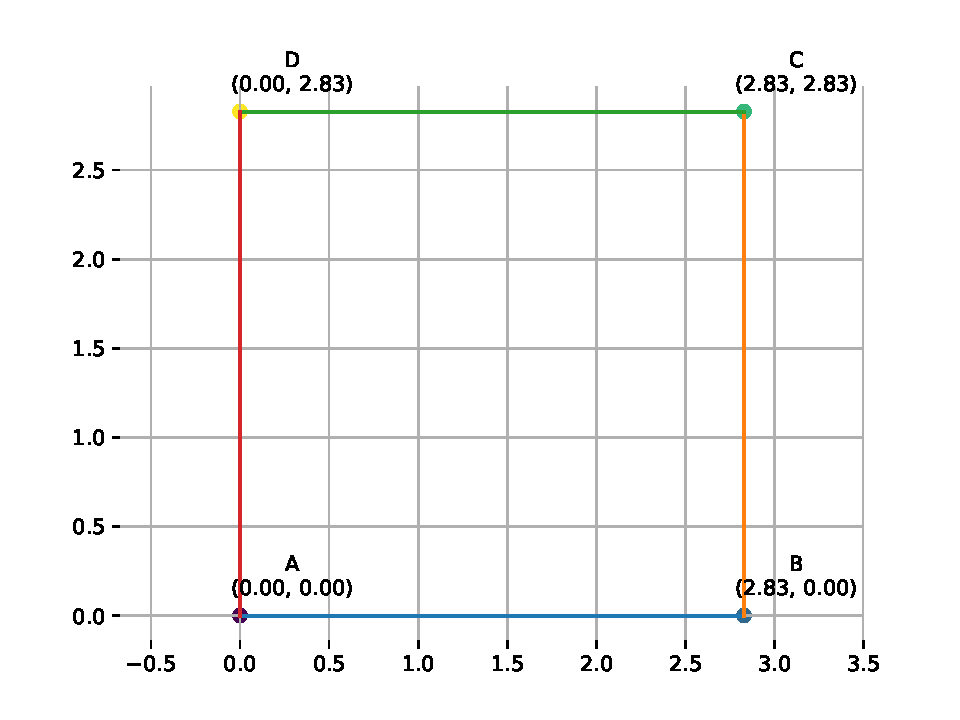
\includegraphics[width=0.75\columnwidth]{chapters/10/7/4/4/figs/fig.pdf}
	\end{center}
\caption{}
\label{fig:7/4/4/4Fig3}
\end{figure}
\begin{figure}[H]
	\begin{center} 
	    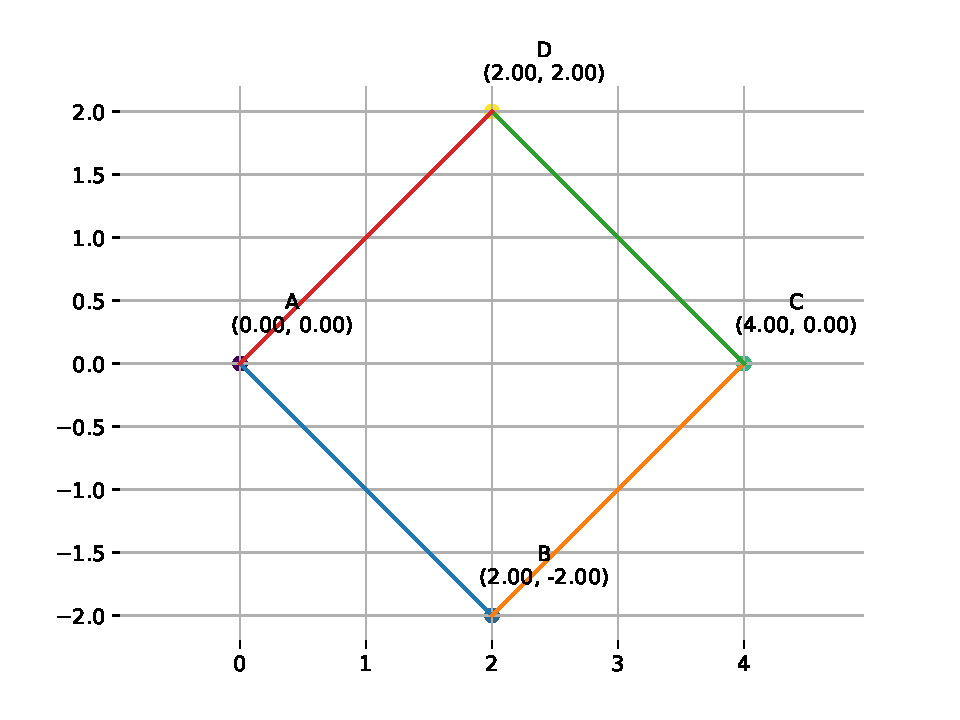
\includegraphics[width=0.75\columnwidth]{chapters/10/7/4/4/figs/fig1.pdf}
	\end{center}
\caption{}
\label{fig:7/4/4/4Fig2}
\end{figure}
\begin{figure}[H]
	\begin{center} 
	    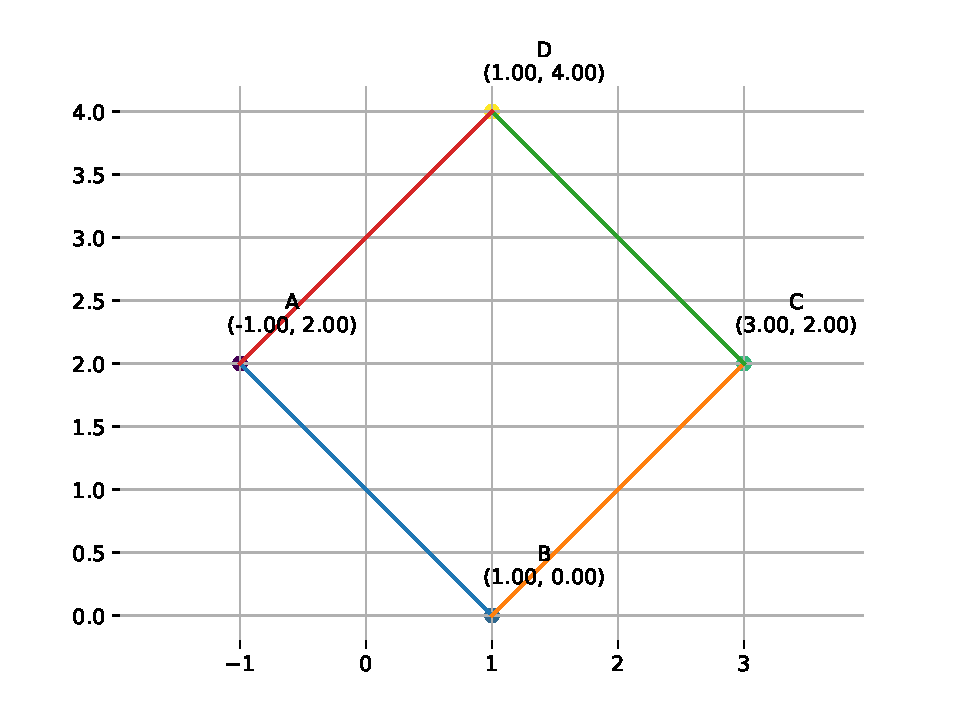
\includegraphics[width=0.75\columnwidth]{chapters/10/7/4/4/figs/fig2.pdf}
	\end{center}
\caption{}
\label{fig:7/4/4/4Fig1}
\end{figure}

\item The base of an equilateral triangle with side $2a$ lies along the y-axis such that the mid-point of the base is at the origin. Find the vertices of the triangle.
\label{chapters/11/10/1/2}
	\\
	\solution 
The direction vector
\begin{align}
	\vec{B}-\vec{A}
	=
	\myvec{
  h-x_1\\
  k-y_1
  }
   \equiv
	\myvec{
1\\
	\frac{ k-y_1}{h-x_1}
  }
  \\
	\implies m = 
	\frac{ k-y_1}{h-x_1},
\end{align}
yielding the desired result.

\item Let $\vec{a}$ and $\vec{b}$ be two unit vectors and $\theta$ the angle between them. Then $\vec{a}+\vec{b}$ is a unit vector if
	\begin{enumerate}
			\itemsep2pt
		\item $\theta = \frac{\pi}{4}$
		\item $\theta = \frac{\pi}{3}$
		\item $\theta = \frac{\pi}{2}$
		\item $\theta = \frac{2\pi}{3}$
			\end{enumerate}
\solution
\begin{align}
	\because \norm{\vec{a}}=\norm{\vec{b}}  = 3 \norm{\vec{a}+\vec{b}}&=1, \label{eq:12/10/5/17/2} \\
    \norm{\vec{a}+\vec{b}}^2 & = 1^2 \\
    \implies \norm{\vec{a}}^2 + \norm{\vec{b}}^2 + 2\vec{a}^{\top}\vec{b} & = 1 \label{eq:12/10/5/17/3} \\
    \implies (\norm{\vec{a}}\norm{\vec{b}}\cos{\theta}) & = \frac{-1}{2} \label{eq:12/10/5/17/4} \\
	\implies \cos{\theta}  = \frac{-1}{2}, \text{or, }\theta&=\frac{2\pi}{3}
\end{align}

\item Show that the tangent of an angle between the lines 
\begin{align}
	\frac{x}{a}+\frac{y}{b}&=1 \text{ and }
	\\
	\frac{x}{a}-\frac{y}{b}&=1 
\end{align}
is $\frac{2ab}{a^2-b^2}$.
\item Find $\abs{\overrightarrow {x}}$, if for a unit vector $\overrightarrow {a}, (\overrightarrow {x}-\overrightarrow {a})\cdot (\overrightarrow {x}+\overrightarrow {a}$)=12.
	\\
\solution 
		From the given information,
		\begin{align}
			\vec{a}=\myvec{\cos\frac{\pi}{3}\\\cos\frac{\pi}{4}\\\cos\theta}
			= 
\myvec{\frac{1}{2}\\[1ex]\frac{1}{\sqrt{2}}\\[1ex]\cos\theta}
		\end{align}
\begin{align}
\because    \norm{\vec{a}}&=1,
\\
\frac{1}{4}+\frac{1}{2}+\cos^2\theta&=1
\\
    \implies\cos\theta &=\frac{1}{2}
\end{align}
$\because \theta$ is an acute angle.
    Hence 
\begin{align}
		\vec{a}=\myvec{\frac{1}{2}\\[1ex] \frac{1}{\sqrt{2}}\\[1ex] \frac{1}{2}}
\end{align}

\item Find $\abs{\overrightarrow {a}}$ and $\abs{\overrightarrow {b}}$, if ($\overrightarrow {a}+\overrightarrow {b})\cdot (\overrightarrow {a}-\overrightarrow {b})=8$ and $\abs{\overrightarrow {a}}=8\abs{\overrightarrow {b}}$.
	\\
	\solution
		From the given information,
		\begin{align}
			\vec{a}=\myvec{\cos\frac{\pi}{3}\\\cos\frac{\pi}{4}\\\cos\theta}
			= 
\myvec{\frac{1}{2}\\[1ex]\frac{1}{\sqrt{2}}\\[1ex]\cos\theta}
		\end{align}
\begin{align}
\because    \norm{\vec{a}}&=1,
\\
\frac{1}{4}+\frac{1}{2}+\cos^2\theta&=1
\\
    \implies\cos\theta &=\frac{1}{2}
\end{align}
$\because \theta$ is an acute angle.
    Hence 
\begin{align}
		\vec{a}=\myvec{\frac{1}{2}\\[1ex] \frac{1}{\sqrt{2}}\\[1ex] \frac{1}{2}}
\end{align}

\item Find the magnitude of two vectors $\overrightarrow {a}$ and $\overrightarrow {b}$, having the same magnitude and such that the angle between them is $60\degree$ and their scalar product is $\frac{1}{2}$.
	\\
	\solution
		\iffalse
\documentclass[journal,12pt,twocolumn]{IEEEtran}
%
\usepackage{setspace}
\usepackage{gensymb}
%\doublespacing
\singlespacing

%\usepackage{graphicx}
%\usepackage{amssymb}
%\usepackage{relsize}
\usepackage[cmex10]{amsmath}
%\usepackage{amsthm}
%\interdisplaylinepenalty=2500
%\savesymbol{iint}
%\usepackage{txfonts}
%\restoresymbol{TXF}{iint}
%\usepackage{wasysym}
\usepackage{amsthm}
%\usepackage{iithtlc}
\usepackage{mathrsfs}
\usepackage{txfonts}
\usepackage{stfloats}
\usepackage{bm}
\usepackage{cite}
\usepackage{cases}
\usepackage{subfig}
%\usepackage{xtab}
\usepackage{longtable}
\usepackage{multirow}
%\usepackage{algorithm}
%\usepackage{algpseudocode}
\usepackage{enumitem}
\usepackage{mathtools}
\usepackage{steinmetz}
\usepackage{tikz}
\usepackage{circuitikz}
\usepackage{verbatim}
\usepackage{tfrupee}
\usepackage[breaklinks=true]{hyperref}
%\usepackage{stmaryrd}
\usepackage{tkz-euclide} % loads  TikZ and tkz-base
%\usetkzobj{all}
\usetikzlibrary{calc,math}
\usepackage{listings}
    \usepackage{color}                                            %%
    \usepackage{array}                                            %%
    \usepackage{longtable}                                        %%
    \usepackage{calc}                                             %%
    \usepackage{multirow}                                         %%
    \usepackage{hhline}                                           %%
    \usepackage{ifthen}                                           %%
  %optionally (for landscape tables embedded in another document): %%
    \usepackage{lscape}     
\usepackage{multicol}
\usepackage{chngcntr}
%\usepackage{enumerate}

%\usepackage{wasysym}
%\newcounter{MYtempeqncnt}
\DeclareMathOperator*{\Res}{Res}
%\renewcommand{\baselinestretch}{2}
\renewcommand\thesection{\arabic{section}}
\renewcommand\thesubsection{\thesection.\arabic{subsection}}
\renewcommand\thesubsubsection{\thesubsection.\arabic{subsubsection}}

\renewcommand\thesectiondis{\arabic{section}}
\renewcommand\thesubsectiondis{\thesectiondis.\arabic{subsection}}
\renewcommand\thesubsubsectiondis{\thesubsectiondis.\arabic{subsubsection}}

% correct bad hyphenation here
\hyphenation{op-tical net-works semi-conduc-tor}
\def\inputGnumericTable{}                                 %%

\lstset{
%language=C,
frame=single, 
breaklines=true,
columns=fullflexible
}
%\lstset{
%language=tex,
%frame=single, 
%breaklines=true
%}


\begin{document}
%


\newtheorem{theorem}{Theorem}[section]
\newtheorem{problem}{Problem}
\newtheorem{proposition}{Proposition}[section]
\newtheorem{lemma}{Lemma}[section]
\newtheorem{corollary}[theorem]{Corollary}
\newtheorem{example}{Example}[section]
\newtheorem{definition}[problem]{Definition}
%\newtheorem{thm}{Theorem}[section] 
%\newtheorem{defn}[thm]{Definition}
%\newtheorem{algorithm}{Algorithm}[section]
%\newtheorem{cor}{Corollary}
\newcommand{\BEQA}{\begin{eqnarray}}
\newcommand{\EEQA}{\end{eqnarray}}
\newcommand{\define}{\stackrel{\triangle}{=}}

\bibliographystyle{IEEEtran}
%\bibliographystyle{ieeetr}


\providecommand{\mbf}{\mathbf}
\providecommand{\pr}[1]{\ensuremath{\Pr\left(#1\right)}}
\providecommand{\qfunc}[1]{\ensuremath{Q\left(#1\right)}}
\providecommand{\sbrak}[1]{\ensuremath{{}\left[#1\right]}}
\providecommand{\lsbrak}[1]{\ensuremath{{}\left[#1\right.}}
\providecommand{\rsbrak}[1]{\ensuremath{{}\left.#1\right]}}
\providecommand{\brak}[1]{\ensuremath{\left(#1\right)}}
\providecommand{\lbrak}[1]{\ensuremath{\left(#1\right.}}
\providecommand{\rbrak}[1]{\ensuremath{\left.#1\right)}}
\providecommand{\cbrak}[1]{\ensuremath{\left\{#1\right\}}}
\providecommand{\lcbrak}[1]{\ensuremath{\left\{#1\right.}}
\providecommand{\rcbrak}[1]{\ensuremath{\left.#1\right\}}}
\theoremstyle{remark}
\newtheorem{rem}{Remark}
\newcommand{\sgn}{\mathop{\mathrm{sgn}}}
\providecommand{\abs}[1]{\left\vert#1\right\vert}
\providecommand{\res}[1]{\Res\displaylimits_{#1}} 
\providecommand{\norm}[1]{\left\lVert#1\right\rVert}
%\providecommand{\norm}[1]{\lVert#1\rVert}
\providecommand{\mtx}[1]{\mathbf{#1}}
\providecommand{\mean}[1]{E\left[ #1 \right]}
\providecommand{\fourier}{\overset{\mathcal{F}}{ \rightleftharpoons}}
%\providecommand{\hilbert}{\overset{\mathcal{H}}{ \rightleftharpoons}}
\providecommand{\system}{\overset{\mathcal{H}}{ \longleftrightarrow}}
	%\newcommand{\solution}[2]{\textbf{Solution:}{#1}}
\newcommand{\solution}{\noindent \textbf{Solution: }}
\newcommand{\cosec}{\,\text{cosec}\,}
\providecommand{\dec}[2]{\ensuremath{\overset{#1}{\underset{#2}{\gtrless}}}}
\newcommand{\myvec}[1]{\ensuremath{\begin{pmatrix}#1\end{pmatrix}}}
\newcommand{\mydet}[1]{\ensuremath{\begin{vmatrix}#1\end{vmatrix}}}
%\numberwithin{equation}{section}
\numberwithin{equation}{subsection}
%\numberwithin{problem}{section}
%\numberwithin{definition}{section}
\makeatletter
\@addtoreset{figure}{problem}
\makeatother

\let\StandardTheFigure\thefigure
\let\vec\mathbf
%\renewcommand{\thefigure}{\theproblem.\arabic{figure}}
\renewcommand{\thefigure}{\theproblem}
%\setlist[enumerate,1]{before=\renewcommand\theequation{\theenumi.\arabic{equation}}
%\counterwithin{equation}{enumi}


%\renewcommand{\theequation}{\arabic{subsection}.\arabic{equation}}

\def\putbox#1#2#3{\makebox[0in][l]{\makebox[#1][l]{}\raisebox{\baselineskip}[0in][0in]{\raisebox{#2}[0in][0in]{#3}}}}
     \def\rightbox#1{\makebox[0in][r]{#1}}
     \def\centbox#1{\makebox[0in]{#1}}
     \def\topbox#1{\raisebox{-\baselineskip}[0in][0in]{#1}}
     \def\midbox#1{\raisebox{-0.5\baselineskip}[0in][0in]{#1}}

\vspace{3cm}


\title{Quiz 4}
\author{S Nithish}





% make the title area
\maketitle

\newpage

%\tableofcontents

\bigskip

\renewcommand{\thefigure}{\theenumi}
\renewcommand{\thetable}{\theenumi}
%\renewcommand{\theequation}{\theenumi}


\begin{abstract}
This document contains the solution of the question from NCERT 11th standard chapter 10 exercise 10.1 problem 7
\end{abstract}

%Download all python codes 
%
%\begin{lstlisting}
%svn co https://github.com/JayatiD93/trunk/My_solution_design/codes
%\end{lstlisting}

%Download all and latex-tikz codes from 
%
%\begin{lstlisting}
%svn co https://github.com/gadepall/school/trunk/ncert/geometry/figs
%\end{lstlisting}
%


\section{Exercise 10.1}

\begin{enumerate}

	\fi
Let the direction vector of the y-axis be
\begin{align}
\vec{m_1} = \myvec{0 \\ 1}
\end{align}
and the direction vector of the line be,
\begin{align}
\vec{m_2} = \myvec{1 \\ m}
\end{align}
where $m$ is the slope of the line.
Then, 
\begin{align}
	\vec{m_1}^{\top} \vec{m_2}   = m, \,
	\norm{\vec{m_1}}   = 1, \,
	\norm{\vec{m_2}}  = \sqrt{1+m^2}
\end{align}
yielding
the angle between the two as
\begin{align}
	\cos (\phi) &= \frac{m}{\sqrt{1+m^2}}
	 = \frac{\sqrt{3}}{2}\\
\implies
	m &= \pm \sqrt{3} 
\end{align}
Thus, 
$m=\sqrt{3}$ is the correct slope.


\item Show that $\abs {\overrightarrow {a}}\overrightarrow {b}+\abs{\overrightarrow {b}}\overrightarrow {a}$ is perpendicular to $\abs{\overrightarrow {a}} \overrightarrow {b}-\abs{\overrightarrow {b}} \overrightarrow {a}$, for any two nonzero vectors $\overrightarrow {a}$ and $\overrightarrow {b}$.
	\\
	\solution
		\iffalse
\documentclass[journal,12pt,twocolumn]{IEEEtran}
%
\usepackage{setspace}
\usepackage{gensymb}
%\doublespacing
\singlespacing

%\usepackage{graphicx}
%\usepackage{amssymb}
%\usepackage{relsize}
\usepackage[cmex10]{amsmath}
%\usepackage{amsthm}
%\interdisplaylinepenalty=2500
%\savesymbol{iint}
%\usepackage{txfonts}
%\restoresymbol{TXF}{iint}
%\usepackage{wasysym}
\usepackage{amsthm}
%\usepackage{iithtlc}
\usepackage{mathrsfs}
\usepackage{txfonts}
\usepackage{stfloats}
\usepackage{bm}
\usepackage{cite}
\usepackage{cases}
\usepackage{subfig}
%\usepackage{xtab}
\usepackage{longtable}
\usepackage{multirow}
%\usepackage{algorithm}
%\usepackage{algpseudocode}
\usepackage{enumitem}
\usepackage{mathtools}
\usepackage{steinmetz}
\usepackage{tikz}
\usepackage{circuitikz}
\usepackage{verbatim}
\usepackage{tfrupee}
\usepackage[breaklinks=true]{hyperref}
%\usepackage{stmaryrd}
\usepackage{tkz-euclide} % loads  TikZ and tkz-base
%\usetkzobj{all}
\usetikzlibrary{calc,math}
\usepackage{listings}
    \usepackage{color}                                            %%
    \usepackage{array}                                            %%
    \usepackage{longtable}                                        %%
    \usepackage{calc}                                             %%
    \usepackage{multirow}                                         %%
    \usepackage{hhline}                                           %%
    \usepackage{ifthen}                                           %%
  %optionally (for landscape tables embedded in another document): %%
    \usepackage{lscape}     
\usepackage{multicol}
\usepackage{chngcntr}
%\usepackage{enumerate}

%\usepackage{wasysym}
%\newcounter{MYtempeqncnt}
\DeclareMathOperator*{\Res}{Res}
%\renewcommand{\baselinestretch}{2}
\renewcommand\thesection{\arabic{section}}
\renewcommand\thesubsection{\thesection.\arabic{subsection}}
\renewcommand\thesubsubsection{\thesubsection.\arabic{subsubsection}}

\renewcommand\thesectiondis{\arabic{section}}
\renewcommand\thesubsectiondis{\thesectiondis.\arabic{subsection}}
\renewcommand\thesubsubsectiondis{\thesubsectiondis.\arabic{subsubsection}}

% correct bad hyphenation here
\hyphenation{op-tical net-works semi-conduc-tor}
\def\inputGnumericTable{}                                 %%

\lstset{
%language=C,
frame=single, 
breaklines=true,
columns=fullflexible
}
%\lstset{
%language=tex,
%frame=single, 
%breaklines=true
%}


\begin{document}
%


\newtheorem{theorem}{Theorem}[section]
\newtheorem{problem}{Problem}
\newtheorem{proposition}{Proposition}[section]
\newtheorem{lemma}{Lemma}[section]
\newtheorem{corollary}[theorem]{Corollary}
\newtheorem{example}{Example}[section]
\newtheorem{definition}[problem]{Definition}
%\newtheorem{thm}{Theorem}[section] 
%\newtheorem{defn}[thm]{Definition}
%\newtheorem{algorithm}{Algorithm}[section]
%\newtheorem{cor}{Corollary}
\newcommand{\BEQA}{\begin{eqnarray}}
\newcommand{\EEQA}{\end{eqnarray}}
\newcommand{\define}{\stackrel{\triangle}{=}}

\bibliographystyle{IEEEtran}
%\bibliographystyle{ieeetr}


\providecommand{\mbf}{\mathbf}
\providecommand{\pr}[1]{\ensuremath{\Pr\left(#1\right)}}
\providecommand{\qfunc}[1]{\ensuremath{Q\left(#1\right)}}
\providecommand{\sbrak}[1]{\ensuremath{{}\left[#1\right]}}
\providecommand{\lsbrak}[1]{\ensuremath{{}\left[#1\right.}}
\providecommand{\rsbrak}[1]{\ensuremath{{}\left.#1\right]}}
\providecommand{\brak}[1]{\ensuremath{\left(#1\right)}}
\providecommand{\lbrak}[1]{\ensuremath{\left(#1\right.}}
\providecommand{\rbrak}[1]{\ensuremath{\left.#1\right)}}
\providecommand{\cbrak}[1]{\ensuremath{\left\{#1\right\}}}
\providecommand{\lcbrak}[1]{\ensuremath{\left\{#1\right.}}
\providecommand{\rcbrak}[1]{\ensuremath{\left.#1\right\}}}
\theoremstyle{remark}
\newtheorem{rem}{Remark}
\newcommand{\sgn}{\mathop{\mathrm{sgn}}}
\providecommand{\abs}[1]{\left\vert#1\right\vert}
\providecommand{\res}[1]{\Res\displaylimits_{#1}} 
\providecommand{\norm}[1]{\left\lVert#1\right\rVert}
%\providecommand{\norm}[1]{\lVert#1\rVert}
\providecommand{\mtx}[1]{\mathbf{#1}}
\providecommand{\mean}[1]{E\left[ #1 \right]}
\providecommand{\fourier}{\overset{\mathcal{F}}{ \rightleftharpoons}}
%\providecommand{\hilbert}{\overset{\mathcal{H}}{ \rightleftharpoons}}
\providecommand{\system}{\overset{\mathcal{H}}{ \longleftrightarrow}}
	%\newcommand{\solution}[2]{\textbf{Solution:}{#1}}
\newcommand{\solution}{\noindent \textbf{Solution: }}
\newcommand{\cosec}{\,\text{cosec}\,}
\providecommand{\dec}[2]{\ensuremath{\overset{#1}{\underset{#2}{\gtrless}}}}
\newcommand{\myvec}[1]{\ensuremath{\begin{pmatrix}#1\end{pmatrix}}}
\newcommand{\mydet}[1]{\ensuremath{\begin{vmatrix}#1\end{vmatrix}}}
%\numberwithin{equation}{section}
\numberwithin{equation}{subsection}
%\numberwithin{problem}{section}
%\numberwithin{definition}{section}
\makeatletter
\@addtoreset{figure}{problem}
\makeatother

\let\StandardTheFigure\thefigure
\let\vec\mathbf
%\renewcommand{\thefigure}{\theproblem.\arabic{figure}}
\renewcommand{\thefigure}{\theproblem}
%\setlist[enumerate,1]{before=\renewcommand\theequation{\theenumi.\arabic{equation}}
%\counterwithin{equation}{enumi}


%\renewcommand{\theequation}{\arabic{subsection}.\arabic{equation}}

\def\putbox#1#2#3{\makebox[0in][l]{\makebox[#1][l]{}\raisebox{\baselineskip}[0in][0in]{\raisebox{#2}[0in][0in]{#3}}}}
     \def\rightbox#1{\makebox[0in][r]{#1}}
     \def\centbox#1{\makebox[0in]{#1}}
     \def\topbox#1{\raisebox{-\baselineskip}[0in][0in]{#1}}
     \def\midbox#1{\raisebox{-0.5\baselineskip}[0in][0in]{#1}}

\vspace{3cm}


\title{Quiz 4}
\author{S Nithish}





% make the title area
\maketitle

\newpage

%\tableofcontents

\bigskip

\renewcommand{\thefigure}{\theenumi}
\renewcommand{\thetable}{\theenumi}
%\renewcommand{\theequation}{\theenumi}


\begin{abstract}
This document contains the solution of the question from NCERT 11th standard chapter 10 exercise 10.1 problem 7
\end{abstract}

%Download all python codes 
%
%\begin{lstlisting}
%svn co https://github.com/JayatiD93/trunk/My_solution_design/codes
%\end{lstlisting}

%Download all and latex-tikz codes from 
%
%\begin{lstlisting}
%svn co https://github.com/gadepall/school/trunk/ncert/geometry/figs
%\end{lstlisting}
%


\section{Exercise 10.1}

\begin{enumerate}

	\fi
Let the direction vector of the y-axis be
\begin{align}
\vec{m_1} = \myvec{0 \\ 1}
\end{align}
and the direction vector of the line be,
\begin{align}
\vec{m_2} = \myvec{1 \\ m}
\end{align}
where $m$ is the slope of the line.
Then, 
\begin{align}
	\vec{m_1}^{\top} \vec{m_2}   = m, \,
	\norm{\vec{m_1}}   = 1, \,
	\norm{\vec{m_2}}  = \sqrt{1+m^2}
\end{align}
yielding
the angle between the two as
\begin{align}
	\cos (\phi) &= \frac{m}{\sqrt{1+m^2}}
	 = \frac{\sqrt{3}}{2}\\
\implies
	m &= \pm \sqrt{3} 
\end{align}
Thus, 
$m=\sqrt{3}$ is the correct slope.


\item If $\vec{a}$, $\vec{b}$, $\vec{c}$ are unit vectors such that $\vec{a}$+$\vec{b}$+$\vec{c}$=0, then the value of $\vec{a} \cdot \vec{b}+\vec{b} \cdot \vec{c}+\vec{c} \cdot \vec{a}$ is
	\begin{enumerate}
\item 1
\item 3
\item $\frac{-3}{2}$
\item None of these
\end{enumerate}
	\solution
		From the given information,
		\begin{align}
			\vec{a}=\myvec{\cos\frac{\pi}{3}\\\cos\frac{\pi}{4}\\\cos\theta}
			= 
\myvec{\frac{1}{2}\\[1ex]\frac{1}{\sqrt{2}}\\[1ex]\cos\theta}
		\end{align}
\begin{align}
\because    \norm{\vec{a}}&=1,
\\
\frac{1}{4}+\frac{1}{2}+\cos^2\theta&=1
\\
    \implies\cos\theta &=\frac{1}{2}
\end{align}
$\because \theta$ is an acute angle.
    Hence 
\begin{align}
		\vec{a}=\myvec{\frac{1}{2}\\[1ex] \frac{1}{\sqrt{2}}\\[1ex] \frac{1}{2}}
\end{align}

\item If either vector $\overrightarrow {a}=0$ or $\overrightarrow {b}=0$, then $\overrightarrow {a}.\overrightarrow {b}$=0. But the converse need not be true. Justify your answer with an example.
	\\
	\solution
		\iffalse
\documentclass[journal,12pt,twocolumn]{IEEEtran}
%
\usepackage{setspace}
\usepackage{gensymb}
%\doublespacing
\singlespacing

%\usepackage{graphicx}
%\usepackage{amssymb}
%\usepackage{relsize}
\usepackage[cmex10]{amsmath}
%\usepackage{amsthm}
%\interdisplaylinepenalty=2500
%\savesymbol{iint}
%\usepackage{txfonts}
%\restoresymbol{TXF}{iint}
%\usepackage{wasysym}
\usepackage{amsthm}
%\usepackage{iithtlc}
\usepackage{mathrsfs}
\usepackage{txfonts}
\usepackage{stfloats}
\usepackage{bm}
\usepackage{cite}
\usepackage{cases}
\usepackage{subfig}
%\usepackage{xtab}
\usepackage{longtable}
\usepackage{multirow}
%\usepackage{algorithm}
%\usepackage{algpseudocode}
\usepackage{enumitem}
\usepackage{mathtools}
\usepackage{steinmetz}
\usepackage{tikz}
\usepackage{circuitikz}
\usepackage{verbatim}
\usepackage{tfrupee}
\usepackage[breaklinks=true]{hyperref}
%\usepackage{stmaryrd}
\usepackage{tkz-euclide} % loads  TikZ and tkz-base
%\usetkzobj{all}
\usetikzlibrary{calc,math}
\usepackage{listings}
    \usepackage{color}                                            %%
    \usepackage{array}                                            %%
    \usepackage{longtable}                                        %%
    \usepackage{calc}                                             %%
    \usepackage{multirow}                                         %%
    \usepackage{hhline}                                           %%
    \usepackage{ifthen}                                           %%
  %optionally (for landscape tables embedded in another document): %%
    \usepackage{lscape}     
\usepackage{multicol}
\usepackage{chngcntr}
%\usepackage{enumerate}

%\usepackage{wasysym}
%\newcounter{MYtempeqncnt}
\DeclareMathOperator*{\Res}{Res}
%\renewcommand{\baselinestretch}{2}
\renewcommand\thesection{\arabic{section}}
\renewcommand\thesubsection{\thesection.\arabic{subsection}}
\renewcommand\thesubsubsection{\thesubsection.\arabic{subsubsection}}

\renewcommand\thesectiondis{\arabic{section}}
\renewcommand\thesubsectiondis{\thesectiondis.\arabic{subsection}}
\renewcommand\thesubsubsectiondis{\thesubsectiondis.\arabic{subsubsection}}

% correct bad hyphenation here
\hyphenation{op-tical net-works semi-conduc-tor}
\def\inputGnumericTable{}                                 %%

\lstset{
%language=C,
frame=single, 
breaklines=true,
columns=fullflexible
}
%\lstset{
%language=tex,
%frame=single, 
%breaklines=true
%}


\begin{document}
%


\newtheorem{theorem}{Theorem}[section]
\newtheorem{problem}{Problem}
\newtheorem{proposition}{Proposition}[section]
\newtheorem{lemma}{Lemma}[section]
\newtheorem{corollary}[theorem]{Corollary}
\newtheorem{example}{Example}[section]
\newtheorem{definition}[problem]{Definition}
%\newtheorem{thm}{Theorem}[section] 
%\newtheorem{defn}[thm]{Definition}
%\newtheorem{algorithm}{Algorithm}[section]
%\newtheorem{cor}{Corollary}
\newcommand{\BEQA}{\begin{eqnarray}}
\newcommand{\EEQA}{\end{eqnarray}}
\newcommand{\define}{\stackrel{\triangle}{=}}

\bibliographystyle{IEEEtran}
%\bibliographystyle{ieeetr}


\providecommand{\mbf}{\mathbf}
\providecommand{\pr}[1]{\ensuremath{\Pr\left(#1\right)}}
\providecommand{\qfunc}[1]{\ensuremath{Q\left(#1\right)}}
\providecommand{\sbrak}[1]{\ensuremath{{}\left[#1\right]}}
\providecommand{\lsbrak}[1]{\ensuremath{{}\left[#1\right.}}
\providecommand{\rsbrak}[1]{\ensuremath{{}\left.#1\right]}}
\providecommand{\brak}[1]{\ensuremath{\left(#1\right)}}
\providecommand{\lbrak}[1]{\ensuremath{\left(#1\right.}}
\providecommand{\rbrak}[1]{\ensuremath{\left.#1\right)}}
\providecommand{\cbrak}[1]{\ensuremath{\left\{#1\right\}}}
\providecommand{\lcbrak}[1]{\ensuremath{\left\{#1\right.}}
\providecommand{\rcbrak}[1]{\ensuremath{\left.#1\right\}}}
\theoremstyle{remark}
\newtheorem{rem}{Remark}
\newcommand{\sgn}{\mathop{\mathrm{sgn}}}
\providecommand{\abs}[1]{\left\vert#1\right\vert}
\providecommand{\res}[1]{\Res\displaylimits_{#1}} 
\providecommand{\norm}[1]{\left\lVert#1\right\rVert}
%\providecommand{\norm}[1]{\lVert#1\rVert}
\providecommand{\mtx}[1]{\mathbf{#1}}
\providecommand{\mean}[1]{E\left[ #1 \right]}
\providecommand{\fourier}{\overset{\mathcal{F}}{ \rightleftharpoons}}
%\providecommand{\hilbert}{\overset{\mathcal{H}}{ \rightleftharpoons}}
\providecommand{\system}{\overset{\mathcal{H}}{ \longleftrightarrow}}
	%\newcommand{\solution}[2]{\textbf{Solution:}{#1}}
\newcommand{\solution}{\noindent \textbf{Solution: }}
\newcommand{\cosec}{\,\text{cosec}\,}
\providecommand{\dec}[2]{\ensuremath{\overset{#1}{\underset{#2}{\gtrless}}}}
\newcommand{\myvec}[1]{\ensuremath{\begin{pmatrix}#1\end{pmatrix}}}
\newcommand{\mydet}[1]{\ensuremath{\begin{vmatrix}#1\end{vmatrix}}}
%\numberwithin{equation}{section}
\numberwithin{equation}{subsection}
%\numberwithin{problem}{section}
%\numberwithin{definition}{section}
\makeatletter
\@addtoreset{figure}{problem}
\makeatother

\let\StandardTheFigure\thefigure
\let\vec\mathbf
%\renewcommand{\thefigure}{\theproblem.\arabic{figure}}
\renewcommand{\thefigure}{\theproblem}
%\setlist[enumerate,1]{before=\renewcommand\theequation{\theenumi.\arabic{equation}}
%\counterwithin{equation}{enumi}


%\renewcommand{\theequation}{\arabic{subsection}.\arabic{equation}}

\def\putbox#1#2#3{\makebox[0in][l]{\makebox[#1][l]{}\raisebox{\baselineskip}[0in][0in]{\raisebox{#2}[0in][0in]{#3}}}}
     \def\rightbox#1{\makebox[0in][r]{#1}}
     \def\centbox#1{\makebox[0in]{#1}}
     \def\topbox#1{\raisebox{-\baselineskip}[0in][0in]{#1}}
     \def\midbox#1{\raisebox{-0.5\baselineskip}[0in][0in]{#1}}

\vspace{3cm}


\title{Quiz 4}
\author{S Nithish}





% make the title area
\maketitle

\newpage

%\tableofcontents

\bigskip

\renewcommand{\thefigure}{\theenumi}
\renewcommand{\thetable}{\theenumi}
%\renewcommand{\theequation}{\theenumi}


\begin{abstract}
This document contains the solution of the question from NCERT 11th standard chapter 10 exercise 10.1 problem 7
\end{abstract}

%Download all python codes 
%
%\begin{lstlisting}
%svn co https://github.com/JayatiD93/trunk/My_solution_design/codes
%\end{lstlisting}

%Download all and latex-tikz codes from 
%
%\begin{lstlisting}
%svn co https://github.com/gadepall/school/trunk/ncert/geometry/figs
%\end{lstlisting}
%


\section{Exercise 10.1}

\begin{enumerate}

	\fi
Let the direction vector of the y-axis be
\begin{align}
\vec{m_1} = \myvec{0 \\ 1}
\end{align}
and the direction vector of the line be,
\begin{align}
\vec{m_2} = \myvec{1 \\ m}
\end{align}
where $m$ is the slope of the line.
Then, 
\begin{align}
	\vec{m_1}^{\top} \vec{m_2}   = m, \,
	\norm{\vec{m_1}}   = 1, \,
	\norm{\vec{m_2}}  = \sqrt{1+m^2}
\end{align}
yielding
the angle between the two as
\begin{align}
	\cos (\phi) &= \frac{m}{\sqrt{1+m^2}}
	 = \frac{\sqrt{3}}{2}\\
\implies
	m &= \pm \sqrt{3} 
\end{align}
Thus, 
$m=\sqrt{3}$ is the correct slope.


\item Prove that $(\vec{a}+\vec{b})\cdot(\vec{a}+\vec{b})=|{\vec{a}}|^2+|{\vec{b}}|^2$, if and only if $\vec{a}, \vec{b}$ are perpendicular, given $\vec{a}\neq\vec{0}, \vec{b}\neq\vec{0}$.\\
	\solution
		\iffalse
\documentclass[journal,12pt,twocolumn]{IEEEtran}
%
\usepackage{setspace}
\usepackage{gensymb}
%\doublespacing
\singlespacing

%\usepackage{graphicx}
%\usepackage{amssymb}
%\usepackage{relsize}
\usepackage[cmex10]{amsmath}
%\usepackage{amsthm}
%\interdisplaylinepenalty=2500
%\savesymbol{iint}
%\usepackage{txfonts}
%\restoresymbol{TXF}{iint}
%\usepackage{wasysym}
\usepackage{amsthm}
%\usepackage{iithtlc}
\usepackage{mathrsfs}
\usepackage{txfonts}
\usepackage{stfloats}
\usepackage{bm}
\usepackage{cite}
\usepackage{cases}
\usepackage{subfig}
%\usepackage{xtab}
\usepackage{longtable}
\usepackage{multirow}
%\usepackage{algorithm}
%\usepackage{algpseudocode}
\usepackage{enumitem}
\usepackage{mathtools}
\usepackage{steinmetz}
\usepackage{tikz}
\usepackage{circuitikz}
\usepackage{verbatim}
\usepackage{tfrupee}
\usepackage[breaklinks=true]{hyperref}
%\usepackage{stmaryrd}
\usepackage{tkz-euclide} % loads  TikZ and tkz-base
%\usetkzobj{all}
\usetikzlibrary{calc,math}
\usepackage{listings}
    \usepackage{color}                                            %%
    \usepackage{array}                                            %%
    \usepackage{longtable}                                        %%
    \usepackage{calc}                                             %%
    \usepackage{multirow}                                         %%
    \usepackage{hhline}                                           %%
    \usepackage{ifthen}                                           %%
  %optionally (for landscape tables embedded in another document): %%
    \usepackage{lscape}     
\usepackage{multicol}
\usepackage{chngcntr}
%\usepackage{enumerate}

%\usepackage{wasysym}
%\newcounter{MYtempeqncnt}
\DeclareMathOperator*{\Res}{Res}
%\renewcommand{\baselinestretch}{2}
\renewcommand\thesection{\arabic{section}}
\renewcommand\thesubsection{\thesection.\arabic{subsection}}
\renewcommand\thesubsubsection{\thesubsection.\arabic{subsubsection}}

\renewcommand\thesectiondis{\arabic{section}}
\renewcommand\thesubsectiondis{\thesectiondis.\arabic{subsection}}
\renewcommand\thesubsubsectiondis{\thesubsectiondis.\arabic{subsubsection}}

% correct bad hyphenation here
\hyphenation{op-tical net-works semi-conduc-tor}
\def\inputGnumericTable{}                                 %%

\lstset{
%language=C,
frame=single, 
breaklines=true,
columns=fullflexible
}
%\lstset{
%language=tex,
%frame=single, 
%breaklines=true
%}


\begin{document}
%


\newtheorem{theorem}{Theorem}[section]
\newtheorem{problem}{Problem}
\newtheorem{proposition}{Proposition}[section]
\newtheorem{lemma}{Lemma}[section]
\newtheorem{corollary}[theorem]{Corollary}
\newtheorem{example}{Example}[section]
\newtheorem{definition}[problem]{Definition}
%\newtheorem{thm}{Theorem}[section] 
%\newtheorem{defn}[thm]{Definition}
%\newtheorem{algorithm}{Algorithm}[section]
%\newtheorem{cor}{Corollary}
\newcommand{\BEQA}{\begin{eqnarray}}
\newcommand{\EEQA}{\end{eqnarray}}
\newcommand{\define}{\stackrel{\triangle}{=}}

\bibliographystyle{IEEEtran}
%\bibliographystyle{ieeetr}


\providecommand{\mbf}{\mathbf}
\providecommand{\pr}[1]{\ensuremath{\Pr\left(#1\right)}}
\providecommand{\qfunc}[1]{\ensuremath{Q\left(#1\right)}}
\providecommand{\sbrak}[1]{\ensuremath{{}\left[#1\right]}}
\providecommand{\lsbrak}[1]{\ensuremath{{}\left[#1\right.}}
\providecommand{\rsbrak}[1]{\ensuremath{{}\left.#1\right]}}
\providecommand{\brak}[1]{\ensuremath{\left(#1\right)}}
\providecommand{\lbrak}[1]{\ensuremath{\left(#1\right.}}
\providecommand{\rbrak}[1]{\ensuremath{\left.#1\right)}}
\providecommand{\cbrak}[1]{\ensuremath{\left\{#1\right\}}}
\providecommand{\lcbrak}[1]{\ensuremath{\left\{#1\right.}}
\providecommand{\rcbrak}[1]{\ensuremath{\left.#1\right\}}}
\theoremstyle{remark}
\newtheorem{rem}{Remark}
\newcommand{\sgn}{\mathop{\mathrm{sgn}}}
\providecommand{\abs}[1]{\left\vert#1\right\vert}
\providecommand{\res}[1]{\Res\displaylimits_{#1}} 
\providecommand{\norm}[1]{\left\lVert#1\right\rVert}
%\providecommand{\norm}[1]{\lVert#1\rVert}
\providecommand{\mtx}[1]{\mathbf{#1}}
\providecommand{\mean}[1]{E\left[ #1 \right]}
\providecommand{\fourier}{\overset{\mathcal{F}}{ \rightleftharpoons}}
%\providecommand{\hilbert}{\overset{\mathcal{H}}{ \rightleftharpoons}}
\providecommand{\system}{\overset{\mathcal{H}}{ \longleftrightarrow}}
	%\newcommand{\solution}[2]{\textbf{Solution:}{#1}}
\newcommand{\solution}{\noindent \textbf{Solution: }}
\newcommand{\cosec}{\,\text{cosec}\,}
\providecommand{\dec}[2]{\ensuremath{\overset{#1}{\underset{#2}{\gtrless}}}}
\newcommand{\myvec}[1]{\ensuremath{\begin{pmatrix}#1\end{pmatrix}}}
\newcommand{\mydet}[1]{\ensuremath{\begin{vmatrix}#1\end{vmatrix}}}
%\numberwithin{equation}{section}
\numberwithin{equation}{subsection}
%\numberwithin{problem}{section}
%\numberwithin{definition}{section}
\makeatletter
\@addtoreset{figure}{problem}
\makeatother

\let\StandardTheFigure\thefigure
\let\vec\mathbf
%\renewcommand{\thefigure}{\theproblem.\arabic{figure}}
\renewcommand{\thefigure}{\theproblem}
%\setlist[enumerate,1]{before=\renewcommand\theequation{\theenumi.\arabic{equation}}
%\counterwithin{equation}{enumi}


%\renewcommand{\theequation}{\arabic{subsection}.\arabic{equation}}

\def\putbox#1#2#3{\makebox[0in][l]{\makebox[#1][l]{}\raisebox{\baselineskip}[0in][0in]{\raisebox{#2}[0in][0in]{#3}}}}
     \def\rightbox#1{\makebox[0in][r]{#1}}
     \def\centbox#1{\makebox[0in]{#1}}
     \def\topbox#1{\raisebox{-\baselineskip}[0in][0in]{#1}}
     \def\midbox#1{\raisebox{-0.5\baselineskip}[0in][0in]{#1}}

\vspace{3cm}


\title{Quiz 4}
\author{S Nithish}





% make the title area
\maketitle

\newpage

%\tableofcontents

\bigskip

\renewcommand{\thefigure}{\theenumi}
\renewcommand{\thetable}{\theenumi}
%\renewcommand{\theequation}{\theenumi}


\begin{abstract}
This document contains the solution of the question from NCERT 11th standard chapter 10 exercise 10.1 problem 7
\end{abstract}

%Download all python codes 
%
%\begin{lstlisting}
%svn co https://github.com/JayatiD93/trunk/My_solution_design/codes
%\end{lstlisting}

%Download all and latex-tikz codes from 
%
%\begin{lstlisting}
%svn co https://github.com/gadepall/school/trunk/ncert/geometry/figs
%\end{lstlisting}
%


\section{Exercise 10.1}

\begin{enumerate}

	\fi
Let the direction vector of the y-axis be
\begin{align}
\vec{m_1} = \myvec{0 \\ 1}
\end{align}
and the direction vector of the line be,
\begin{align}
\vec{m_2} = \myvec{1 \\ m}
\end{align}
where $m$ is the slope of the line.
Then, 
\begin{align}
	\vec{m_1}^{\top} \vec{m_2}   = m, \,
	\norm{\vec{m_1}}   = 1, \,
	\norm{\vec{m_2}}  = \sqrt{1+m^2}
\end{align}
yielding
the angle between the two as
\begin{align}
	\cos (\phi) &= \frac{m}{\sqrt{1+m^2}}
	 = \frac{\sqrt{3}}{2}\\
\implies
	m &= \pm \sqrt{3} 
\end{align}
Thus, 
$m=\sqrt{3}$ is the correct slope.


	\item  If $l_1, m_1,n_1 \text{ and } l_2,m_2,n_2$ are the direction cosines of two mutually perpendicular lines, show that the direction cosines of the line perpendicular to both these are  $m_1n_2-m_2n_1,n_1l_2-n_2l_1,l_1m_2-l_2m_1$.
\\
    \solution
		\iffalse
\documentclass[journal,12pt,twocolumn]{IEEEtran}
%
\usepackage{setspace}
\usepackage{gensymb}
%\doublespacing
\singlespacing

%\usepackage{graphicx}
%\usepackage{amssymb}
%\usepackage{relsize}
\usepackage[cmex10]{amsmath}
%\usepackage{amsthm}
%\interdisplaylinepenalty=2500
%\savesymbol{iint}
%\usepackage{txfonts}
%\restoresymbol{TXF}{iint}
%\usepackage{wasysym}
\usepackage{amsthm}
%\usepackage{iithtlc}
\usepackage{mathrsfs}
\usepackage{txfonts}
\usepackage{stfloats}
\usepackage{bm}
\usepackage{cite}
\usepackage{cases}
\usepackage{subfig}
%\usepackage{xtab}
\usepackage{longtable}
\usepackage{multirow}
%\usepackage{algorithm}
%\usepackage{algpseudocode}
\usepackage{enumitem}
\usepackage{mathtools}
\usepackage{steinmetz}
\usepackage{tikz}
\usepackage{circuitikz}
\usepackage{verbatim}
\usepackage{tfrupee}
\usepackage[breaklinks=true]{hyperref}
%\usepackage{stmaryrd}
\usepackage{tkz-euclide} % loads  TikZ and tkz-base
%\usetkzobj{all}
\usetikzlibrary{calc,math}
\usepackage{listings}
    \usepackage{color}                                            %%
    \usepackage{array}                                            %%
    \usepackage{longtable}                                        %%
    \usepackage{calc}                                             %%
    \usepackage{multirow}                                         %%
    \usepackage{hhline}                                           %%
    \usepackage{ifthen}                                           %%
  %optionally (for landscape tables embedded in another document): %%
    \usepackage{lscape}     
\usepackage{multicol}
\usepackage{chngcntr}
%\usepackage{enumerate}

%\usepackage{wasysym}
%\newcounter{MYtempeqncnt}
\DeclareMathOperator*{\Res}{Res}
%\renewcommand{\baselinestretch}{2}
\renewcommand\thesection{\arabic{section}}
\renewcommand\thesubsection{\thesection.\arabic{subsection}}
\renewcommand\thesubsubsection{\thesubsection.\arabic{subsubsection}}

\renewcommand\thesectiondis{\arabic{section}}
\renewcommand\thesubsectiondis{\thesectiondis.\arabic{subsection}}
\renewcommand\thesubsubsectiondis{\thesubsectiondis.\arabic{subsubsection}}

% correct bad hyphenation here
\hyphenation{op-tical net-works semi-conduc-tor}
\def\inputGnumericTable{}                                 %%

\lstset{
%language=C,
frame=single, 
breaklines=true,
columns=fullflexible
}
%\lstset{
%language=tex,
%frame=single, 
%breaklines=true
%}


\begin{document}
%


\newtheorem{theorem}{Theorem}[section]
\newtheorem{problem}{Problem}
\newtheorem{proposition}{Proposition}[section]
\newtheorem{lemma}{Lemma}[section]
\newtheorem{corollary}[theorem]{Corollary}
\newtheorem{example}{Example}[section]
\newtheorem{definition}[problem]{Definition}
%\newtheorem{thm}{Theorem}[section] 
%\newtheorem{defn}[thm]{Definition}
%\newtheorem{algorithm}{Algorithm}[section]
%\newtheorem{cor}{Corollary}
\newcommand{\BEQA}{\begin{eqnarray}}
\newcommand{\EEQA}{\end{eqnarray}}
\newcommand{\define}{\stackrel{\triangle}{=}}

\bibliographystyle{IEEEtran}
%\bibliographystyle{ieeetr}


\providecommand{\mbf}{\mathbf}
\providecommand{\pr}[1]{\ensuremath{\Pr\left(#1\right)}}
\providecommand{\qfunc}[1]{\ensuremath{Q\left(#1\right)}}
\providecommand{\sbrak}[1]{\ensuremath{{}\left[#1\right]}}
\providecommand{\lsbrak}[1]{\ensuremath{{}\left[#1\right.}}
\providecommand{\rsbrak}[1]{\ensuremath{{}\left.#1\right]}}
\providecommand{\brak}[1]{\ensuremath{\left(#1\right)}}
\providecommand{\lbrak}[1]{\ensuremath{\left(#1\right.}}
\providecommand{\rbrak}[1]{\ensuremath{\left.#1\right)}}
\providecommand{\cbrak}[1]{\ensuremath{\left\{#1\right\}}}
\providecommand{\lcbrak}[1]{\ensuremath{\left\{#1\right.}}
\providecommand{\rcbrak}[1]{\ensuremath{\left.#1\right\}}}
\theoremstyle{remark}
\newtheorem{rem}{Remark}
\newcommand{\sgn}{\mathop{\mathrm{sgn}}}
\providecommand{\abs}[1]{\left\vert#1\right\vert}
\providecommand{\res}[1]{\Res\displaylimits_{#1}} 
\providecommand{\norm}[1]{\left\lVert#1\right\rVert}
%\providecommand{\norm}[1]{\lVert#1\rVert}
\providecommand{\mtx}[1]{\mathbf{#1}}
\providecommand{\mean}[1]{E\left[ #1 \right]}
\providecommand{\fourier}{\overset{\mathcal{F}}{ \rightleftharpoons}}
%\providecommand{\hilbert}{\overset{\mathcal{H}}{ \rightleftharpoons}}
\providecommand{\system}{\overset{\mathcal{H}}{ \longleftrightarrow}}
	%\newcommand{\solution}[2]{\textbf{Solution:}{#1}}
\newcommand{\solution}{\noindent \textbf{Solution: }}
\newcommand{\cosec}{\,\text{cosec}\,}
\providecommand{\dec}[2]{\ensuremath{\overset{#1}{\underset{#2}{\gtrless}}}}
\newcommand{\myvec}[1]{\ensuremath{\begin{pmatrix}#1\end{pmatrix}}}
\newcommand{\mydet}[1]{\ensuremath{\begin{vmatrix}#1\end{vmatrix}}}
%\numberwithin{equation}{section}
\numberwithin{equation}{subsection}
%\numberwithin{problem}{section}
%\numberwithin{definition}{section}
\makeatletter
\@addtoreset{figure}{problem}
\makeatother

\let\StandardTheFigure\thefigure
\let\vec\mathbf
%\renewcommand{\thefigure}{\theproblem.\arabic{figure}}
\renewcommand{\thefigure}{\theproblem}
%\setlist[enumerate,1]{before=\renewcommand\theequation{\theenumi.\arabic{equation}}
%\counterwithin{equation}{enumi}


%\renewcommand{\theequation}{\arabic{subsection}.\arabic{equation}}

\def\putbox#1#2#3{\makebox[0in][l]{\makebox[#1][l]{}\raisebox{\baselineskip}[0in][0in]{\raisebox{#2}[0in][0in]{#3}}}}
     \def\rightbox#1{\makebox[0in][r]{#1}}
     \def\centbox#1{\makebox[0in]{#1}}
     \def\topbox#1{\raisebox{-\baselineskip}[0in][0in]{#1}}
     \def\midbox#1{\raisebox{-0.5\baselineskip}[0in][0in]{#1}}

\vspace{3cm}


\title{Quiz 4}
\author{S Nithish}





% make the title area
\maketitle

\newpage

%\tableofcontents

\bigskip

\renewcommand{\thefigure}{\theenumi}
\renewcommand{\thetable}{\theenumi}
%\renewcommand{\theequation}{\theenumi}


\begin{abstract}
This document contains the solution of the question from NCERT 11th standard chapter 10 exercise 10.1 problem 7
\end{abstract}

%Download all python codes 
%
%\begin{lstlisting}
%svn co https://github.com/JayatiD93/trunk/My_solution_design/codes
%\end{lstlisting}

%Download all and latex-tikz codes from 
%
%\begin{lstlisting}
%svn co https://github.com/gadepall/school/trunk/ncert/geometry/figs
%\end{lstlisting}
%


\section{Exercise 10.1}

\begin{enumerate}

	\fi
Let the direction vector of the y-axis be
\begin{align}
\vec{m_1} = \myvec{0 \\ 1}
\end{align}
and the direction vector of the line be,
\begin{align}
\vec{m_2} = \myvec{1 \\ m}
\end{align}
where $m$ is the slope of the line.
Then, 
\begin{align}
	\vec{m_1}^{\top} \vec{m_2}   = m, \,
	\norm{\vec{m_1}}   = 1, \,
	\norm{\vec{m_2}}  = \sqrt{1+m^2}
\end{align}
yielding
the angle between the two as
\begin{align}
	\cos (\phi) &= \frac{m}{\sqrt{1+m^2}}
	 = \frac{\sqrt{3}}{2}\\
\implies
	m &= \pm \sqrt{3} 
\end{align}
Thus, 
$m=\sqrt{3}$ is the correct slope.


\item
Find the angle between the lines whose direction ratios are $a,b,c$ and $b-c,c-a,a-b$.
\\
\solution
    \begin{align}
\because \myvec{a&b&c}\myvec{b-c\\c-a\\a-b} = 0,
   \theta=\frac{\pi}{2}
    \end{align}

\item The value of the expression $\abs{\vec{a}\times\vec{b}}$+ $({\vec{a}\cdot\vec{b}})$ is \rule{1cm}{0.15mm}
\item If $\abs{\vec{a}\times\vec{b}}^2$ + $\abs{\vec{a}\cdot\vec{b}}^2$=144 $\text{and}$  $\abs{\vec{a}}$=4, then $\abs{\vec{b}}$ is equal to \rule{1cm}{0.15mm}.
\item If the directions cosines of a line are $(k,k,k)$ then
\begin{enumerate}
	\item $k>0$
	\item $0<k<1$
	\item $k=1$ 
	\item $k=\dfrac{1}{\sqrt{3}}$ or $-\dfrac{1}{\sqrt{3}}$
\end{enumerate}
\item  Find the position vector of a point A in space such that $\overrightarrow{OA}$ is inclined at $60 \degree$ to OX and at $45 \degree$ to OY and $\abs{\overrightarrow{OA}} =10$ units.
\item If $(-4,3)\text{ and }(4,3)$ are two vertices of an equilateral triangle. Find the coordinates of the third vertex, given that the origin lies in the interior of the triangle. 
\item $\vec{A} (6,1),\vec{B}(8,2) \text{ and } \vec{C}(9,4)$ are three vertices of a parallelogram ABCD. If $\vec{C}$ is the midpoint of DC find the area of $\triangle ADE$.
\item If the points  $\vec{A}(1,-2), \vec{B}(2,3) , \vec{C}(a,2)\text{ and }\vec{D} (-4-3)$ form parallelogram, find the value of $a$ and height of the parallelogram taking AB as base.
\item Ayush starts walking from his house to office. Instead of going to the office directly, he goes to a bank first, from there to his daughter school and then reaches the office what is the extra distance travelled by Ayush in reaching his office? If the house is situated at $(2,4)$, bank at $(5,8)$, school at $(13,14)$ and office at $(13,26)$ and coordinates are in km.
\item Find the angle between the lines whose direction cosines are given by the equations $l+m+n=0$, $l^2+m^2-n^2=0$.
\item If a variable line in two adjacent positions has directions cosines $l, m, n$ and $l+\delta l, m+\delta m, n+\delta n$, show that the small angle $\delta\theta$ between the two positions is given by 
\begin{align}
	\delta\theta^2=\delta l^2+\delta m^2+\delta n^2
\end{align}
\item The vector $\vec{a}+\vec{b}$ bisects the angle between the non-collinear vectors $\vec{a}$ $\text{ and }$ $\vec{b}$ if \rule{1cm}{0.15mm}.
\item If $\vec{a}$ $\text{ and }$ $\vec{b}$ are adjacent sides of a rhombus, then $\vec{a}\cdot \vec{b}$=0.
    \item If $ \vec{A},\vec{B},\vec{C} $ are mutually perpendicular vectors of equal magnitudes,show that the  $ \vec{A}+\vec{B}+\vec{C} $ is equally inclined to $ \vec{A},\vec{B}  \text{ and }  \vec{C} $.
\item Projection vector of $\vec{a}$ on $\vec{b}$ is
	\begin{enumerate}
\item $\left(\frac{\vec{a}\cdot\vec{b}}{\abs{\vec{b}}^2}\right)$
\item $\frac{\vec{a}\cdot\vec{b}}{\abs{\vec{b}}}$
\item $\frac{\vec{a}\cdot\vec{b}}{\abs{\vec{a}}}$
\item $\left(\frac{\vec{a}\cdot\vec{b}}{\abs{\vec{a}}^2}\right)$
\end{enumerate}
\item If $\vec{a}$ is  any non-zero vector, then $(\vec{a}\cdot \hat{i})\hat{i}$+$(\vec{a}\cdot \hat{j})\hat{j}$+$(\vec{a}\cdot \hat{k})$ $\hat{k}$ equals \rule{1cm}{0.15mm}.
\item If $\vec{a},\vec{b},\vec{c}$ are the three vectors such that $\vec{a}+\vec{b}+\vec{c}=0$ $\text{ and }$ $|\vec{a}|=2$, $|\vec{b}|$=3, $|\vec{c}|$=5, the value of $\vec{a} \cdot \vec{b}+\vec{b} \cdot \vec{c}+\vec{c} \cdot \vec{a}$ is
	\begin{enumerate}
\item 0
\item 1	
\item -19
\item 38
\end{enumerate}
\item If $\vec{r}\cdot\vec{a}=0, \vec{r}\cdot\vec{b}=0$ and $\vec{r}\cdot\vec{c}=0$ for some non-zero vector $\vec{r}$, then the value of $\vec{a}\cdot(\vec{b}\times\vec{c})$ is \rule{1cm}{0.15mm}.
\item If $\abs{\vec{a}+\vec{b}}$ = $\abs{\vec{a}-\vec{b}}$, then the vectors $\vec{a}$ $\text {and}$ $\vec{b}$ are orthogonal.
\item Prove that the lines $x=py+q , z=ry+s \text{ and } x=p^{\prime}y+q^{\prime}, z=r^{\prime}y+s^{\prime} $ are perpendicular if $pp^{\prime}+rr^{\prime}+1=0$.
\item Show that the straight lines whose direction cosines are given by $2l+2m-n=0$ and $mn+nl+lm=0$ are at right angles.
\item If $l_1, m_1, n_1;l_2, m_2, n_2;l_3, m_3, n_3$ are the direction cosines of the three mutually perpendcular lines, prove that the line whose direction cosines are propotional to $l_1+l_2+l_3 , m_1+m_2,m_3, n_1+n_2+n_3$ make angles with them.
\item Assuming that straight lines work as the plane mirror for a point, find the image of the point $(1,2)$ in the line $x-3y+4=0$.
\item Find $\abs{\overrightarrow{a}-\overrightarrow{b}}$, if two vectors $\overrightarrow{a}$ and $\overrightarrow{b}$ are such that $\abs{\overrightarrow{a}}=2, \abs{\overrightarrow{b}}=3$ and $\overrightarrow{a} \cdot \overrightarrow{b}=4$.
\item If $\overrightarrow{a}$ is a unit vector and $(\overrightarrow{x}-\overrightarrow{a}) \cdot (\overrightarrow{x}+\overrightarrow{a})=8$, then find $\abs{\overrightarrow{x}}$.
\item Let $\overrightarrow{a}, \overrightarrow{b},$ and $ \overrightarrow{c}$ are three vectors such that $\abs{\overrightarrow{a}}=3, \abs{\overrightarrow{b}}=4 \abs{\overrightarrow{c}}=5$ and each one of them being perpndicular to the sum of the other to, find $\abs{\overrightarrow{a}+\overrightarrow{b}+\overrightarrow{c}}$.
\item If with reference to the right handed system of mutually perpendicular unit vectors $\hat{i},\hat{j}$ and $\hat{k}, \overrightarrow{\alpha} = 3\hat{i} -\hat{j}, \overrightarrow{\beta}= 2\hat{i} +\hat{j} -3\hat{k}$, then express $\overrightarrow{\beta}$ in the form $\overrightarrow{\beta} = \overrightarrow{\beta_1} +\overrightarrow{\beta_2}$ where $\overrightarrow{\beta_1}$ is parallel to $\overrightarrow{\alpha}$ and $\overrightarrow{\beta_2}$ is perpendicular to $\overrightarrow{\alpha}$.
\item Three vectors $\overrightarrow{a}, \overrightarrow{b}$ and $\overrightarrow{c}$ satisfy the condition $\overrightarrow{a} +\overrightarrow{b} +\overrightarrow{c} =0$. Evaluate the quantity $\mu = \overrightarrow{a}\cdot \overrightarrow{b} +\overrightarrow{b} \cdot \overrightarrow{c} +\overrightarrow{c} \cdot \overrightarrow{a}$, if $\abs{\overrightarrow{a}}=3, \abs{\overrightarrow{b}}=4$ and $\abs{\overrightarrow{c}}=2$. 
\item A line makes angles $\alpha, \beta, \gamma$ and $\delta$  with the diagonals of a cube, prove that 
\begin{align}
\cos^2\alpha +\cos^2\beta +\cos^2\gamma +\cos^2\delta = \frac{4}{3}.
\end{align}
\end{enumerate}
